\documentclass[times, doublespace]{simauth}%For paper submission
%\documentclass[times]{simauth}
% Packages
\usepackage{mdframed}
\usepackage{subcaption}
\usepackage{subfig}
\usepackage{url}
\usepackage{color}
%\usepackage[T1]{fontenc}
%\usepackage{times}
%\usepackage{bm}
%\usepackage{mathtime}

% Customised Commands
\newtheorem{theorem}{Theorem}[section]
\newtheorem{corollary}{Corollary}[theorem]
\newtheorem{lemma}[theorem]{Lemma}
\newenvironment{proof}[1][Proof]{\begin{trivlist}
\item[\hskip \labelsep {\bfseries #1}]}{\end{trivlist}}
\newcommand{\qed}{\nobreak \ifvmode \relax \else
      \ifdim\lastskip<1.5em \hskip-\lastskip
      \hskip1.5em plus0em minus0.5em \fi \nobreak
      \vrule height0.75em width0.5em depth0.25em\fi}

% Bibliographystyle
\bibliographystyle{wileyj}

\begin{document}
\runninghead{Extending statistical models for the source attribution of zoonotic diseases}
\title{Extending statistical models for source attribution of zoonotic diseases: A study of campylobacteriosis} 
\author{Sih-Jing Liao\affil{a},
Jonathan Marshall\affil{a}\corrauth\ \footnotemark[2], Martin L. Hazelton\affil{a} and Nigel P. French\affil{b}}
\address{\affilnum{a} Institute of Fundamental Sciences-Statistics, Massey University, Palmerston North, New Zealand\\
\affilnum{b} mEpiLab, Hopkirk Research Institute, Massey University, Palmerston North, New Zealand}
\corraddr{Jonathan Marshall, Institute of Fundamental Sciences-Statistics, Massey University, Private Bag 11222, Palmerston North, New Zealand\\ \footnotemark[2] E-mail: J.C.marshall@massey.ac.nz}

\begin{abstract}

Preventing and controlling zoonoses through the design and implementation of public health policies requires a thorough understanding of transmission pathways. Modeling jointly the epidemiological data and genetic information on the microbial isolates derived from cases provides a methodology for tracing back the source of infection. The isolate genetic information and the epidemiological data may be modeled at a variety of levels. In this paper, the attribution probability for human cases of campylobacteriosis for each source, conditional on the extent to which each case resides in a rural compared to urban environment, is estimated. A model that incorporates genetic data and evolutionary processes is applied alongside a newly developed genetic data-free model. We show that the inference from each model is comparable except for rare microbial genotypes, and that the effect of ``rurality'' may be modeled linearly on the logit scale, with increasing rurality leading to increasing likelihood of ruminant-sourced campylobacteriosis.

\end{abstract}

\keywords{source attribution; \textit{Campylobacter}; genetic model; Dirichlet prior; HPD interval; DIC}
\maketitle

\section{Introduction}
Modeling of disease surveillance data to explore patterns of infectious diseases has had a long history in public health. Infectious diseases can cause high economic and medical costs due to morbidity and mortality. In recent decades, the annual number of global deaths caused by infections has leveled off at approximate 15 million and may remain at this level for the next three decades \cite{DyeC, WHOM}. In order for such an enormous health burden to be reduced, preventing and controlling infectious diseases becomes extraordinarily important, which depends on how much we know about the nature of disease transmission. For zoonotic diseases, where transmission to humans from animal reservoirs may be via food, water, through environmental contamination or via direct contact with animals, knowledge of the potential sources and pathways of infection is key to reducing the burden of disease. Quantifying the burden of illness attributable to each pathway and source provides valuable information to health professionals making decisions on public health policy for disease control. 

Over the last few decades there have been many models developed for the analysis of zoonotic diseases. Epidemiological models make use of the incidence of cases and geographic data to capture the main characteristics of disease spread. For example, the Susceptible-Infectious-Recovered model \cite{Kerm} classifies populations into a susceptible, infective and recovered status enabling an estimation of the number of individuals who are likely to be infected. Also, models with a combination of spatial and temporal data enable the prediction of the time frame and areas where a disease outbreak is likely to occur \cite{HeldL, Hoehl, Simo}. However zoonotic transmission from animals to humans may be complex, involving many sources and exposures linked by differing pathways. For instance, infected wild birds may contaminate environmental water and cause disease spread to water users, either humans or other animals \cite{Wagen}. Tracing the source of infection is thus crucial to increasing the ability to implement risk management and intervention \cite{Wilso, Morel}. In terms of statistical analysis, modeling zoonoses requires an advanced approach with the focus changed from just epidemiology to a combination of epidemiology, evolutionary genetics and biology \cite{Muell}. Hence, some source attribution models have been proposed to estimate the number of cases attributable to different sources by utilizing epidemiological information and the association with genotypes found in humans and sources \cite{vanP, Hald, MullA}. 

\begin{table}
  \begin{center}
    \begin{tabular}{crrrrrrr}
      \toprule
      ST & \textit{asp} & \textit{gln} & \textit{glt} & \textit{gly} & \textit{pgm}& \textit{tkt}& \textit{unc}\\ \midrule
      45  & 4 & 7 & 10 & 4 & 1 & 7 & 1\\
      474 & 2 & 4 & 1 & 2 & 2 & 1 & 5 \\
      \bottomrule
    \end{tabular}
  \end{center}
  \caption{The allelic profile of genotypes ST-45 and ST-474 is composed of seven allele numbers at each of the seven loci.}
  \label{tab0}
\end{table}

The genetic information used in such integrated models is typically derived from molecular genotyping that groups closely related organisms together \cite{Cotta}. Typically molecular typing methods, such as multilocus sequence typing (MLST) \cite{Dingl, Coll, Urwin} might be used, which utilizes nucleotide sequences of internal fragments of a small set of housekeeping genes. Such sequences have sufficient variation to distinguish differing pathogen lineages, while being relatively stable within lineages. Each unique nucleotide sequence (allele) at each housekeeping gene (locus) is assigned a number, and the set of numbers across all loci (the allelic profile) is then taken as the genotype, with is usually also assigned a number.

For the pathogen \textit{Campylobacter} which causes campylobacteriosis, a worldwide gastrointestinal disease in humans, the commonly used 7-gene MLST scheme consists of housekeeping genes \textit{asp}A (aspartase A), \textit{gln}A (glutamine synthetase), \textit{glt}A (citrate synthase), \textit{gly}A (serine hydroxymethyltransferase), \textit{pgm} (phosphoglucomutase), \textit{tkt} (transketolase), and \textit{unc}A (ATP synthase $\alpha$ subunit). An illustrative example of MLST data for \emph{Campylobacter jejuni} is presented in Table~(\ref{tab0}). It shows that the genotypes ST-45 and ST-474 have different allelic combinations across the seven loci. The different allelic profiles enable comparison of gene similarities or dissimilarities so that an association between sources and infected cases can be made, by comparing the distribution of genotypes from human cases with those from potential reservoirs.

The first step for attribution models that utilize genetic information is building the sampling distribution of genotypes among each putative source. This may range from using the proportion of each observed genotype \cite{Hald} on each source through to utilizing allelic profile information to derive mutation and recombination rates within each source, and migration rates between each source \cite{Wilso}. A key question is whether more complex genetic models yield superior attribution results or whether a significantly simpler model may suffice, but few authors in the literature have addressed this point. This becomes more important as model complexity extends to include epidemiological covariates. We are therefore motivated to develop a simple model in order to assess the additional information that the more complex models provide.

In this paper we develop statistical models for the source attribution, and use a case study of human campylobacteriosis conducted in New Zealand \cite{Marsh} as a demonstration. Human campylobacteriosis is caused mainly by \textit{C. jejuni} and \textit{C. coli} which are the dominant species associated with 80\% and approximately 15\% of illnesses, respectively \cite{Guert}. The common symptoms of infection are diarrhea, abdominal pain and fever. However, a severe complication named Guillain Barre syndrome may develop, which is a life-threatening disease that weakens the nervous system and leads to paralysis in limbs and respiration \cite{Hanha}. The pathogen can be spread between animals, or from animals and wild birds to humans. The transmission route can be via drinking contaminated water, eating undercooked animal food products, or handling animal food products that are already contaminated by faeces. In this study, we compare the performance of the asymmetric Island model \cite{Wilso}, which considers genetic evolution when estimating the genotype sampling distribution on each source, to a simple model that utilizes only the prevalence of each type to derive the sampling distribution. We then extend both models to incorporate covariates such as rurality indicating the area where a human case resides, exploring the effect of human case rurality on attribution results, modeling attribution by rurality using a linear trend on the logit scale or using separate categories in a Bayesian context, and performing model comparison.

\section{Models for source attribution with and without microbial genetic information}
\subsection{Notation and assumptions}
The ultimate goal of attribution models is to estimate the probability that the observed human cases arise from each putative source. Our data comprise microbial genotype information from each observed human case obtained from analysis of stool samples, and also from a pool of non-human cases corresponding to potential zoonotic sources of disease

Given this genotyping information, we first estimate the sampling distribution of genotypes for each source, and then estimate the appropriate combinations of those genotype distributions that most likely give rise to the set of genotypes observed among human cases. Specifying first the sampling distribution of genotypes found on sources is fundamental for the purpose of not only exploring how it affects the source attribution probability, but also investigating the difference in attribution effect made between the model with genetic information and the model without it.

Suppose we have isolates collected from human and non-human cases, of which $H$ isolates belong to humans, and the remaining $N$ isolates are categorized in $J$ groups as the major sources attributed to the infection. Let $I$ genotypes be the total number of unique sequence types (STs) detected from all isolates, and denote $n_j$ as the marginal frequency of STs found in source $j$, where $\sum_j^J n_j = N$. Typically, the number of detected STs $I$ is smaller than the sample size of isolates as multiple isolates will be of the same type.

The likelihood of observing human cases with types $\text{ST}_1, \text{ST}_2, \ldots \text{ST}_H$ follows a multinomial distribution, which via the law of total probability may be expressed as
\begin{align}
  L\Big(\text{ST}_1, \text{ST}_2, \cdots, \text{ST}_H \Big)=\prod_{h=1}^{H}\sum_{j=1}^{J} p\Big(\text{ST}_h \vert \text{source } j\Big) p\Big(\text{source }j\Big),
  \label{Olikh}
\end{align}
where $p(\text{ST}_h \vert \text{source }j)$ is the probability that $\text{ST}_h$ arises from the sampling distribution of source $j$, and $p(\text{source }j)$ is the attribution probability that a random human case is infected from source $j$. Given we know $p(\text{ST}_h \vert \text{source }j)$, estimation of $p(\text{source }j)$ may be found by optimising the likelihood \eqref{Olikh}, for example using a Metropolis Hastings algorithm within a Bayesian context, with suitable priors on $p(\text{source }j)$.

The asymmetric Island model \cite{Wilso} adopted in the source attribution study for human campylobacteriosis \cite{Marsh} utilizes the allelic profile information for each genotype in an evolutionary model, estimating mutation and recombination probabilities within, and migration probabilities between, each source `island'. It thus estimates $p(\text{ST}_h \vert \text{source }j)$ indirectly, by first estimating the evolutionary parameters, and then deriving the sampling distributions. This allows the asymmetric Island model to estimate the likelihood of observing a genotype on a source when it has not been previously observed.

To discover the effect of incorporating genetic information at the allelic profile level as used in the asymmetric Island model, a simple model is developed for the genotype sampling distribution. With the assumption that the observed distribution of genotypes is representative of the true distribution, we model observed genotypes using a multinomial distribution. Let $x_{ij}$ denote the count of ST-$i$ found in source $j$ with the probability $\pi_{ij}$, where $i=1, \ldots, I$ and $j=1, \ldots, J$. To make inference about $\pi_{ij}$, the likelihood is of a multinomial form,
\begin{align}
        L(\boldsymbol{\pi}_{j} ; \boldsymbol{x}_{j}) & = \frac{n_j!}{\prod_{i=1}^{I} x_{ij}!} \prod_{i=1}^I \pi_{ij}^{x_{ij}}, \notag
\end{align}
where $x_{ij}$ can be $0$, indicating STs are yet observed on the sources; $n_j=\sum_{i=1}^I x_{ij}$ is the total count of ST found on source $j$ and $\pi_{ij}$ is subject to $\sum_{i=1}^I \pi_{ij} =1$, and $0 \leq \pi_{ij} \leq 1$. As the family of Dirichlet distributions is a conjugate pair for the multinomial distribution, assume the prior for $\boldsymbol{\pi}_{j}$ follows a Dirichlet density with parameters $\boldsymbol{\alpha}_{j}$,
\begin{align}
  p(\boldsymbol{\pi}_{j}) & \propto \prod_{i=1}^{I}\pi_{ij}^{\alpha_{ij}-1}. \notag
\end{align}
Then the posterior for $\boldsymbol{\pi}_{j}$ takes the form of a Dirichlet probability function with parameters $(\boldsymbol{\alpha}_{j}+\boldsymbol{x}_{j}-\boldsymbol{1})$,
\begin{align}
        p(\boldsymbol{\pi}_{j} \vert \boldsymbol{x}_{j} ) & \propto L(\boldsymbol{\pi}_{j} ; \boldsymbol{x}_{j}) p(\boldsymbol{\pi}_{j}) \notag \\ 
       & \propto \prod_{i=1}^{I}\pi_{ij}^{\alpha_{ij} + x_{ij}-1}, \quad \alpha_{ij} >0. \notag
 \end{align}
To express the belief that every isolate is equally likely \emph{apriori}, the parameter of the Dirichlet prior is assumed as $\boldsymbol{\alpha}_{j}=\boldsymbol{1}$. Therefore, $p(\text{ST}_h \vert \text{source }j)$, $\boldsymbol{X}$) can be obtained by simulating from the Dirichlet posterior.

Lastly, to estimate the attribution probability, 500 samples are taken from $p(\text{ST}_h \vert \text{source }j)$ generated by the asymmetric Island or simple models. For each posterior sample, we make inferences for $p(\text{source }j)$ using the likelihood~\eqref{Olikh}. This has the effect of integrating over the uncertainty in $p(\text{ST}_h \vert \text{source }j)$ when estimating $p(\text{source }j)$.

\subsection{Campylobacteriosis data}

The source attribution study described here uses MLST data collected in the Manawatu region of New Zealand from March, 2005 to December, 2014. The sampling was carried out over the same time period and from the same geographical location, providing $H+N=3,480$ isolates taken from human and non-human cases, $H=1,400$ of which are from humans. The non-human isolates are sampled from chicken carcasses, cattle, sheep, environmental water, wild birds, and so on, we therefore put them into four groups representing major sources of infection: poultry, ruminants, water and others. The total number of unique STs typed from all isolates is $I=355$, and 35\% of genotypes are found among human cases. Table~(\ref{tab1}) lists five common genotypes found in human and source isolates. The first four genotypes are frequently observed in human cases. For four sources, ST-45 and ST-474 are commonly detected in poultry, while ST-42 and ST-61 are typically found in ruminants. Some studies also discover that human cases with ST-45 or ST-474 are likely attributable to poultry, whereas human cases with ST-42 or ST-61 are more likely attributable to ruminants \cite{Muell, Coll, Cart}. Furthermore, it also shows that there are no observations of ST-2381 in humans, poultry or ruminants, indicating that the genotype may only appear in the water or wild birds.

The data also contain two location variables: one is binary, the other is categorical. The binary variable specifies whether a typed human case is from urban or rural areas, whereas the categorical variable further splits up the areas into seven levels. The levels are highly rural/remote area, rural area with low urban influence, rural area with moderate urban influence, rural area with high urban influence, independent urban area, satellite urban area and main urban area. Table~(\ref{tab2}) lists the number of typed human cases in each classification of rurality. The degree of rurality is a set of integers with a range of [-3,3] corresponding to each defined geographical level. Overall, more than 70\% of typed cases lived in urban areas, and approximately 7.5\% of individuals have no information about the location. We will neglect the missing data in the following analysis by assuming that these cases are randomly missing. Further, the table tells us that the population in 2006 and 2013 for each defined area \cite{Stat1, Stat2} is quite stable. We then calculate the infection rate per 100,000 population and illustrate the prevalence in urban and rural areas from 2006 to 2014 in Figure~(\ref{fig1}). The Figure excludes the year of 2005 because the estimates population of both areas is unavailable and the data of typed human cases are incomplete for the entire year. As illustrated in the Figure, the infection rates in 2006 are about 60 and 85 in urban and rural areas, respectively. We notice that the burden of infection in both areas drop remarkably in 2008, resulting from an intervention in the poultry industry implemented by the New Zealand Food Safety Authority (NZFSA) in 2007 and 2008. It shows the intervention improved infection rates in urban areas, however, it only has a temporary effect in rural areas.

\begin{table}
  \begin{center}
    \begin{tabular}{rrrrrr}
      \toprule
      ST & Human & Poultry & Ruminants & Water & Others\\ \midrule
      42 & 54 & 7 & 52 & 10 & 2\\
      45  & 141 & 154 & 10 & 21 & 54\\
      61 & 64 & 7 & 54 & 2 & 1\\
      474 & 239 & 60 & 15 & 5 & 7\\
      2381 & 0 & 0 & 0 & 21 & 3\\
      \bottomrule
    \end{tabular}
  \end{center}
  \caption{The frequency of five genotypes found from human and four source isolates.}
  \label{tab1}
\end{table}

\begin{table}
%  \begin{threeparttable}
  \centering
      \begin{tabular}{rlrrrr}
        \toprule
        Rurality scale & Description & Human cases & 2006 & 2013 \\ \midrule
        -3 & Highly rural/remote area & 19 & 1,572 & 1,527\\
        -2 & Rural area with low urban influence & 92 & 8,373 & 8,304\\
        -1 & Rural area with moderate urban influence & 127 & 10,392 & 10,734\\
        0 & Rural area with high urban influence & 70 & 6,579 & 7,155\\
        1 & Independent urban area & 230 & 28,611 & 28,188\\
        2 & Satellite urban area & 178 & 19,725 & 20,525\\
        3 & Main urban area & 579 & 76,047 & 78,108\\
        \bottomrule
      \end{tabular}
      \caption{Each category of rurality is defined along with the respective number of human cases typed during 2005 and 2014, and the population size in 2006 and 2013, in the Manawatu region of New Zealand.}
      \label{tab2}     
\end{table}


\begin{figure}
  \centering
  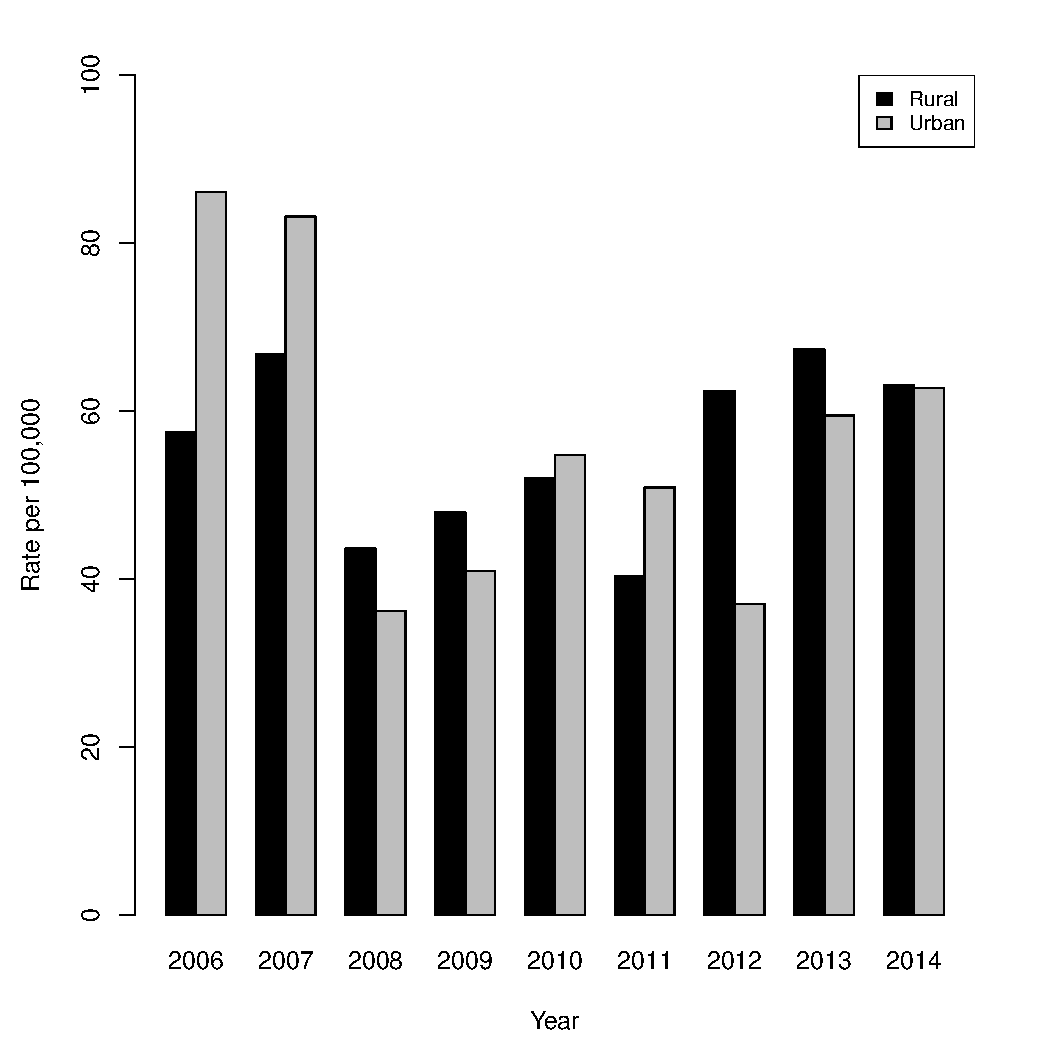
\includegraphics[width=.5\linewidth]{Figures/Databar}
  \caption{The rate per 100,000 population given the typed human cases and the population coming from urban or rural areas in the Manawatu region of New Zealand during 2006 and 2014. A poultry intervention conducted in 2007 and 2008 resulted in a decreasing incidence of campylobacteriosis in the following years, particularly in urban areas.}
  \label{fig1}
\end{figure}

\section{Model fitting for source attribution on rurality scale}

\subsection{Incorporating covariates}

Previously we described how to estimate the marginal probabilities that a randomly selected human case is due to a given source. To extend this analysis so as to include individual level covariates, we need to calculate subject-specific attribution (conditional) probabilities. To that end, let $F_{jh}$ denote the attribution probability of source $j$ for the $h^\textrm{th}$ human case, with constraints $\sum_{j=1}^J F_j =1$ and $0 \leq F_j \leq 1$, where $j=1, \ldots, J$. We model the probabilities $F_{jh}$ using a linear model on the logit scale, that is,  
\begin{align}
  F_{jh}  = \frac{\exp (f_{jh})}{\sum_{j=1}^4 \exp(f_{jh})},
  \label{capF}
\end{align}
where $f_{4h}=0$ is treated as the baseline of $f_{jh}$. Consider the case where the ST data for each human case is supplemented by $p$ additional variables. We develop a general model of $f_{jh}$ with linear combinations of the variables, $c_1, \ldots, c_p$. The model for the $h^\textrm{th}$ individual is then of the form
\begin{align}
f_{jh}  = \alpha_{j} + \beta_{j1} c_{1h} + \beta_{j2} c_{2h} + \ldots + \beta_{jp} c_{ph},  \notag
\end{align}
so that more covariates can be considered in the model to further investigate how the attribution is associated with the factors of interest. Note that if there is a single categorical variable with $L$ levels, then $F_{jh}$ and $f_{jh}$ will take no more than $L$ distinct values. In a slight abuse of notation, we will at times refer to $F_{jh}$ in which the $h$ index refers to the factor level, rather than to a particular subject at that level.

To apply the general model of $f_{jh}$ to the campylobacteriosis data, assume $z$ is the categorical variable representing the classified location of each human case. Then two ways of treating the variable $z$ in model fitting are proposed: one is to treat it as numeric, and the other as categorical. To differentiate the performance between the two fitted models, we link ``the linear model'' and ``the categorical model'' to the first and the latter fitted model, respectively. Hence, the linear prediction function for source $j$ for each human case given the degree of rurality is a numeric variable and can be written as
\begin{align}
  f_{jh} = \alpha_{j} + \beta_{j} z_{h},
  \label{modL}
\end{align}
where $z_{h}$ can be any number of the seven scales if case $h$ was from such a degree of rurality. Conversely, if we treat each of the seven rurality degrees as an indicator with a superscript number $d$, which corresponds with the position of the category ranged from -3 to 3, the model~\eqref{modL} can be rewritten as
\begin{equation}
  f_{jh} = \beta_{1j} z_{1h}+ \beta_{2j} z_{2h} + \ldots + \beta_{dj} z_{dh} + \ldots +  \beta_{7j} z_{7h},
  \label{modC}
\end{equation}
where
\begin{equation*}
z_{dh} =
\left\{\begin{array}{rcl}
1 && \mbox{if case $h$ is in the category $d$,} \notag \\ 0 && \mbox{otherwise}. 
\end{array}\right.
\end{equation*}
As a consequence, the estimated attribution probabilities are obtained via equation~\eqref{capF} after fitting the data to model~\eqref{modL} or to model~\eqref{modC}.

\subsection{MCMC algorithm}
In the interest of quantifying the uncertainty of the posterior attribution probability, we perform Bayesian inference for source attribution probabilities using Markov chain Monte Carlo (MCMC) methods. Assume the priors on parameters of interest in model~\eqref{modL} and model~\eqref{modC} follow a standard normal distribution. Let $\boldsymbol{\theta}$ denote the vector of parameters, with elements $\theta_{t}$ for $t=1, \ldots, T$. For example, $\boldsymbol{\theta}=\{\alpha_1, \alpha_2, \alpha_3, \beta_1, \beta_2, \beta_3\}$ in model~\eqref{modL} or $\boldsymbol{\theta}=\{\beta_{11}, \beta_{12}, \ldots, \beta_{dj}, \ldots, \beta_{73}\}$ in model~\eqref{modC}. We use the Metropolis-Hastings algorithm to update $\theta_{(t)}$ and hence $f_{jh}$ and $ F_{jh}$, in a Markov chain with a length of 30,000 iterations. The first 5,000 samples are removed as the burn-in period (during which time the chain converges) and the sequence is thinned every 10$^{th}$ sample to reduce computer storage. Here are the steps in detail:

\begin{enumerate}
\setcounter{enumi}{-1}
\item Sample $T$ random values from $N(0,1)$ as the initial values points of the parameter set $\boldsymbol{\theta}$ for model~\eqref{modL} or model~\eqref{modC}.
\item Sample a permutation $P_T$ of $\{1, \ldots, T\}$.\label{algorithm_loop}
\item For each $t \in P_T$:
\begin{enumerate}
\item Propose a candidate $\boldsymbol{\theta}^*$ with $\theta_{(t)}$ updated by a normal proposal distribution, $N(\theta_{(t)}, 1)$

\item Use $\boldsymbol{\theta}^*$ to calculate a new set of $f^*$ for source $j$, $j=1, 2, 3$, via model~\eqref{modL} or model~\eqref{modC}, and find the associated $F^*$ for each case by putting the vector $(f^*, f_4=0)$ in equation~\eqref{capF}

\item Compute the acceptance probability $\alpha$, a product of the likelihood ratio, the proposal ratio and the prior ratio, given by
\begin{align*}
\alpha=\frac{L\Big(F^*; \text{ST}, \boldsymbol{Z}\Big)}{L\Big(F; \text{ST}, \boldsymbol{Z}\Big)}\frac{Q\Big(\theta_{(t)} \vert \theta_{(t)}^*\Big)}{Q\Big(\theta_{(t)}^* \vert \theta_{(t)}\Big)}\frac{p\Big(\theta_{(t)}^*\Big)}{p\Big(\theta_{(t)}\Big)}, 
\end{align*}
where the likelihood $L\Big(F^*; \text{ST}, \boldsymbol{Z}\Big)$ involves the rurality covariate $\boldsymbol{Z}$ resulting from the attribution probability, $p(\text{source }j\vert \boldsymbol{Z}$) with an assumption that the genotype distribution on sources is independent of the covariate.
\item Sample $u$ from $U(0,1)$. If $\alpha$ meets $u < \min \left\{1, \alpha \right\}$, in the next state the current proposals of $f^{(*)}$, $F^{(*)}$ and $L\Big(F^{(*)}; \text{ST}, \boldsymbol{Z}\Big)$ are updated; otherwise, the previous proposals are retained.
\end{enumerate}
\item Repeat from step \ref{algorithm_loop} for the given number of iterations.

\end{enumerate}

\section{Results}

\begin{figure}
\centering
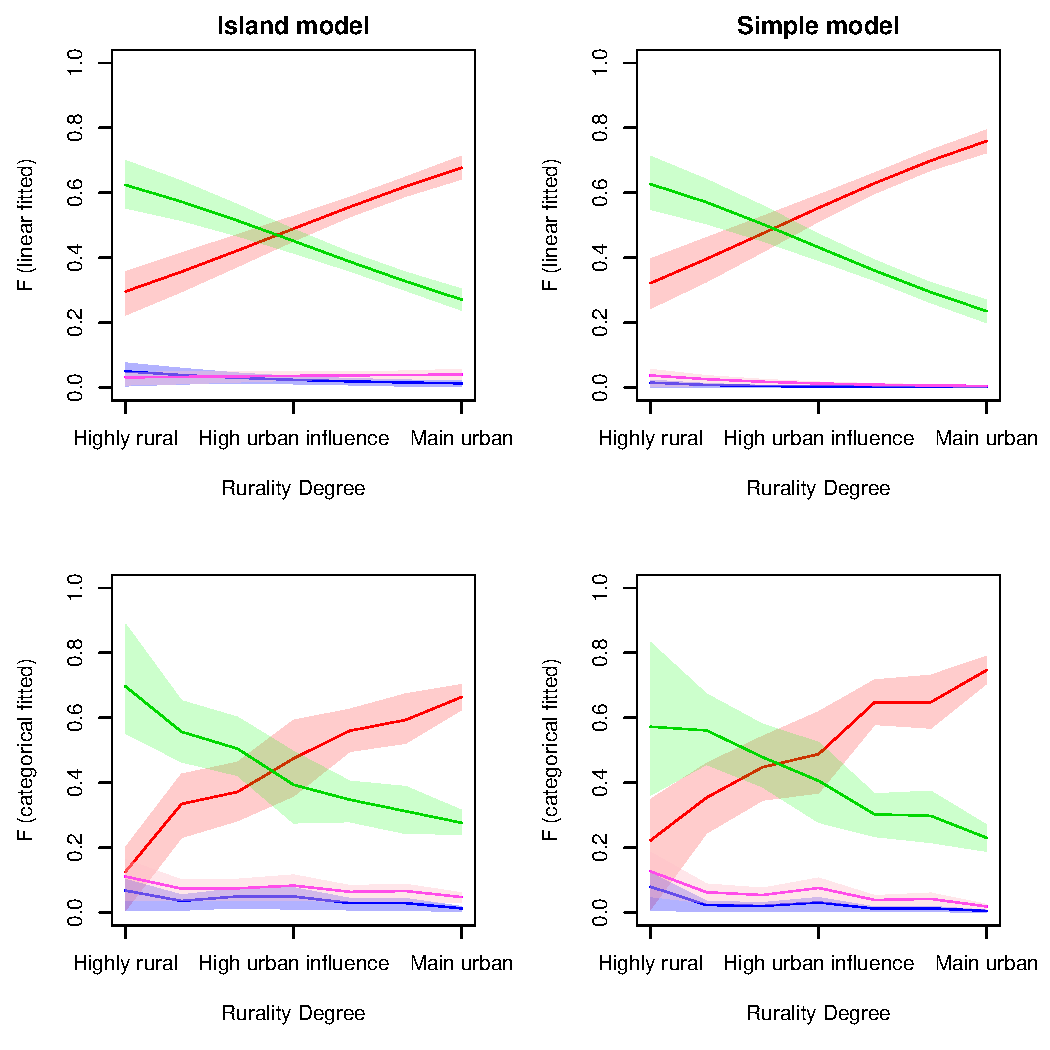
\includegraphics[width=.9\linewidth]{Figures/FCILandC(5)}
\caption{The posterior mean of samples $F$ with 80\% HPD interval for source: poultry (red), ruminants (green), water (blue) and others (pink) over the rurality scales from highly rural area to main urban area. The samples of attribution probability are generated from the two respective fitted models: the linear model (upper panel) and the categorical model (lower panel), given the sampling distribution of genotypes with evolutionary information (the asymmetric Island model) or without any genetic information (the simple model).}
\label{fig2}
\end{figure}

\begin{figure}
\centering
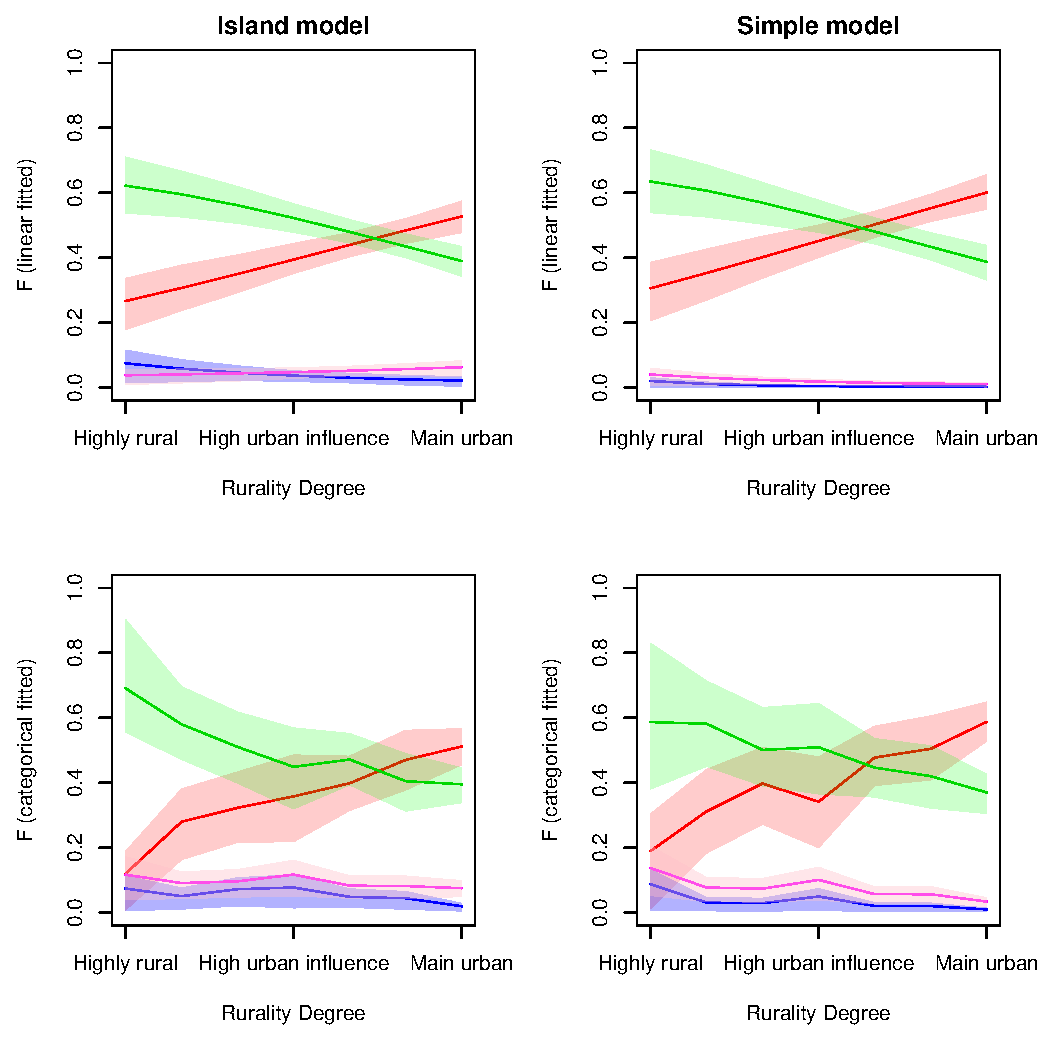
\includegraphics[width=.9\linewidth]{Figures/FCILandC(8)}
\caption{The posterior mean of samples $F$ with 80\% HPD interval for four sources over seven rurality categories after applying our methods to data with the post-intervention time period from 2008 to 2014. The samples of attribution probability are generated from the two respective fitted models -- the linear model (upper panel) and the categorical model (lower panel) -- given the genotype distribution based upon the asymmetric Island model or the simple model.}
\label{fig3}
\end{figure}

To investigate the association between source attribution and human infection, we apply the methods demonstrated in the preceding sections to the campylobacteriosis data and also rearrange the data frame from the ST-based structure to the case-based one for model fitting. The posterior mean of samples $F$ with the 80\% highest posterior density (HPD) interval for each source is illustrated on each rurality grade in Figure~(\ref{fig2}). Given different genotype distributions, the upper panel of the figure is based on the linear model, whereas the lower panel is generated from the categorical model.

For the linear model, the simple model estimates 75\% and 32\% of cases dwelling in main urban areas have acquired the infection from poultry and ruminants, respectively, whereas the asymmetric Island model provides less than 70\% and approximately 30\% of cases attributable to the respective source. Further, the 80\% HPD interval of $F$ for poultry and for ruminants based on the simple model seems marginally wider than that for the asymmetric Island model. So, there is no significant difference in the proportion of human cases attributed to each source between the asymmetric Island and the simple models. For the categorical model, the comparison between the asymmetric Island and the simple models is quite similar to that for the linear model except for the distinguishable attribution for poultry and ruminants in highly rural areas and the much wider credible intervals of $F$ for four sources. For the two fitted models, the narrower credible intervals noticed in very rural areas from the asymmetric Island model might indicate that the asymmetric Island model gives a little more accurate sampling distribution for poultry and ruminants genotypes especially typed in humans living in rural areas. Further, the relatively larger credible intervals observed in the categorical model might be the effect of allocating the number of cases to each qualitative scale (as a dummy variable), particularly in rural areas due to small observations.

Figure~(\ref{fig2}) shows that poultry starts becoming the dominant source contributable to the infection between rural areas with moderate and with high urban influence. In contrast, ruminants are becoming the most attributable source when locations are getting farther away from rural areas with a moderate urban influence. As to water and other sources, they seem to be less influenced by the rurality levels because the probabilities remain less than 0.2 over the seven categories.

Moreover, with a view to examining the robustness of our results, the approach is also applied to data with the time period of post-intervention from 2008 to 2014. The source attribution at different rurality levels is then illustrated in Figure~(\ref{fig3}), displaying that the overall attribution over four sources is moderately consistent with the patterns we previously discovered. However, Figure~(\ref{fig3}) shows a marked decline of attribution probability for poultry and a small rise in probability for ruminants in main urban areas. Despite the fact that the intervention did not eliminate the infection arising from poultry \cite{MuelM}, the reduction highlights the significant improvement in contribution of poultry to the disease, particularly in urban areas where most cases lived. 

Lastly, we use deviance information criterion (DIC) for model comparison. DIC values obtained from our MCMC runs are displayed in Table~\ref{tab3}. Overall there is a clear signal that a linear representation of rurality (on the logit scale) is adequate. Note that the asymmetric Island and Dirichlet models are not directly comparable by DIC as the likelihoods are on different scales: the Dirichlet model assumes all potential sequence types have been observed so that $\sum_j p(\boldsymbol{\pi}_j) = 1$, whereas the asymmetric Island model allows for unobserved sequence types so that $\sum_j p(\boldsymbol{\pi}_j) < 1$.

\begin{table}
  \begin{center}
    \begin{tabular}{crrrrr}
      \toprule
      & \multicolumn{2}{c}{Island model}  & \multicolumn{1}{c}{} & \multicolumn{2}{c}{Dirichlet model} \\
      Data & Linear & Categorical & & Linear & Categorical\\ \midrule
      whole period  & 7913.6 & 7943.3  & & 10328.4  & 10389.8 \\
      post-intervention period  & 5413.4  & 5439.5  & & 6615.1   & 6668.9 \\
      \bottomrule
    \end{tabular}
  \end{center}
  \caption{DIC values for the linear model and for the categorical model applied to the data from 2005 to 2014 (whole period) and to the data from 2008 to 2014 (post-intervention period) given the genotypic information is from the asymmetric Island model or the Dirichlet model.}
  \label{tab3}
\end{table}

\section{Discussions}
Models that determine the source of human infection, particularly with zoonotic pathogens that originate in animal populations, are of considerable value to public health policy-makers. However, the complexity of model building may increase because of the complex transmission pathways of pathogens, in particular when the model combines the epidemiological and molecular data. But, is it necessary to use more complex genetic models for the source attribution of zoonoses? There is limited research on whether using a simpler model could work as effective as complex genetic models. Here we developed a relatively simple model to estimate the attribution probability for each source of \textit{Campylobacter} infection. This model differs to the asymmetric Island model, it does not model the pathogenic evolution but uses a simple genetic classification such as a sequence type of each isolate to illustrate the sampling distribution of genotypes. With the aim of filling the research gap, our results showed that the simple model can do at least similar work, compared to the asymmetric Island model.

In light of the different estimates of the sampling distribution of genotypes from the asymmetric Island and the simple models, two approaches of model fitting (linear and non-linear) were utilized to estimate the attribution probability via the Metropolis-Hastings algorithm. Under the assumption of a logit scale on the attribution probability, we examined how the values of $f$ affected the resulting attribution probability. We changed the standard deviation of the prior distribution from 1 to 2 in the algorithm. The associated posterior mean of attribution probability for each source was invariant despite the fact that the proposals of $f$ jumped even wider in the random walk. This is because the denominator of the equation~\eqref{capF} balances the impact made by the values of $f$. Further, we included a rurality covariate in the model fitting. Our findings not only coincided with the hypothesis that poultry is the major cause of human campylobacteriosis in urban areas \cite{MullA, Marsh, MullM, Leve} but also revealed the linear geographic effect on the infection. It means that poultry is less likely responsible for the infection when cases dwell away from urban areas. Furthermore, the result of decreasing poultry contribution in main urban areas from fitting the data with post-intervention period accorded with what Sears A. and other researchers investigated the effect of poultry intervention \cite{AnnS}. This could provide additional information that would help policy-makers to target interventions to populations residing in urban compared to rural areas.

In conclusion, the simple model is comparable to the asymmetric Island model. The potential of the inclusion of covariates in the model could be applied to help make a decision on the control of the infection. In addition, the simple model (although based on the genetic data) does not capture the evolutionary processes that could be also applied to any type of classification such as phenotype in the research of interest. Nonetheless, there is some concern to apply our approach. One is the role of water that has been recently addressed in the literature \cite{Wagen} by treating it as a medium instead in the transmission network. The other is the larger pathogen datasets resulted from rapidly evolving molecular tools such as the extending MLST schemes typing from seven loci to whole-genome MLST. Hence, reconsidering the role of water as a source of infection and selecting the invaluable information from such large pathogenic data to fit the extended model will be the potential challenges in future research.

\section*{Acknowledgements}

\bibliography{BibArt}

\end{document}
